\documentclass{standalone}
\usepackage{tikz}
\usepackage{ctex,siunitx}
\setCJKmainfont{Noto Serif CJK SC}
\usepackage{tkz-euclide}
\usepackage{amsmath,mhchem}
\usetikzlibrary{patterns, calc}
\usetikzlibrary {decorations.pathmorphing, decorations.pathreplacing, decorations.shapes,}
\begin{document}
% \small
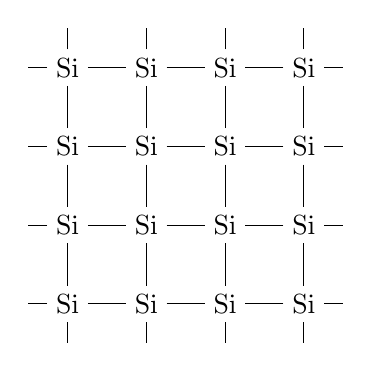
\begin{tikzpicture}[>=stealth,scale=1.0,inner sep=3pt]
  % \useasboundingbox(-1,-2)rectangle(8,6);
  \foreach \x in {1,...,4}
  {
    \foreach \y in {1,...,4}
    {
      \node (si\x\y) at (\x,\y){\ce{Si}};
      \draw (si\x\y)--++(0,0.5);
      \draw (si\x\y)--++(0,-0.5);
      \draw (si\x\y)--++(-0.5,0);
      \draw (si\x\y)--++(0.5,0);
    }
  }
\end{tikzpicture}
\end{document}